%\documentclass[iop]{emulateapj-rtx4}
% \shortauthors{French $\&$ Wakker}
%
%\usepackage{graphicx}
%\usepackage{subfigure}
%\usepackage{hyperref}
%\usepackage{amsmath}


%%%%%%%%%%
\documentclass[twocolumn,tighten]{aastex62}
%\documentclass{aastex6}
%\usepackage{emulateapj-rtx4}
%\usepackage{emulateapj}

 \shortauthors{French $\&$ Wakker}
\usepackage{graphicx}
\usepackage{subfigure}
\usepackage{amsmath}

%\usepackage{dblfloatfix}

%\usepackage{longtable}
%\usepackage{deluxetable}


\newcommand{\kms}{$\rm km\, s^{-1}$}
\newcommand{\HI}{\mbox{H\,{\sc i}} }

%\newcommand{\HI}{H\,{\sc i}}


\newcommand{\I}{\,{\sc i}}
\newcommand{\II}{\,{\sc ii}}
\newcommand{\III}{\,{\sc iii}}
\newcommand{\IV}{\,{\sc iv}}
\newcommand{\V}{\,{\sc v}}
\newcommand{\VI}{\,{\sc vi}}


\graphicspath{{figures//}}

\begin{document}

%\title{The environmental dependence of low-$z$ Ly$\alpha$ absorption}
\title{THE ENVIRONMENTAL DEPENDENCE OF LOW-$z$ LY$\alpha$ ABSORPTION}


%Do Ly$\alpha$ absorbers co-rotate with galaxies?}

\author{David M. French, Bart P. Wakker}

\affil{Department of Astronomy, University of Wisconsin, Madison, WI 53706, USA}

\begin{abstract}
We present the results of a large-scale study of the Ly$\alpha$-probed CGM of nearby galaxies. We have identified 1135 Ly$\alpha$ absorbers in the spectra of 264 background QSOs in the redshift range $0 \leq z \leq 0.033$, and correlated their positions with the surrounding galaxy environment. This has produced a sample of \textbf{XXXX} Ly$\alpha$ component-galaxy pairs, representing the largest-to-date dataset of it's kind. By employing the likelihood-based matching scheme of \cite{french2017}, we quantify the absorber-galaxy spacial correlation and identify 4 distinct absorber sub-samples based on their relative isolation from surrounding galaxies. We find that absorber equivalent width and Doppler-b parameter are enhanced with increasing proximity to galaxies.

\end{abstract}


\keywords{galaxies:intergalactic medium, galaxies:evolution, galaxies:halos, quasars: absorption lines}


\section{INTRODUCTION}

The relationship between high column-density \HI absorption ($N(\HI) \gtrsim 10^{14} ~\rm cm^{-2}$) and galaxies has been well studied in the past several decades (e.g., \citealt{lanzetta1995, bowen1998, bowen2002, chen2003, chen2008, steidel2010, prochaska2011b}). \textbf{What do these studies find?} Relatively few studies have probed the $\rm Ly\alpha$-forest - galaxy relationship below this column density however (e.g., \citealt{wakker2009, french2017, bowen2002}). The most obvious reason for this is due to the technically demanding nature of detecting these weak absorption systems. The installation of the Cosmic Origins Spectrograph (COS) on the Hubble Space Telescope (\emph{HST}) in ??2011?? however has finally opened a window to study this rich reservoir of intergalactic gas.  Thanks to the high throughput and sensitivity available with COS, a large number of distant quasi-stellar objects (QSOs) have been observed with sufficiently high signal-to-noise for a large variety of science priorities. 

...


The second major challenge for galaxy-absorber correlation studies is obtaining data on the galaxies. While the resolution of absorption line spectroscopy is redshift-independent (e.g., a $N(\HI) \gtrsim 10^{13}  ~\rm cm^{-2}$ $\rm Ly\alpha$ absorber is just as readily detected at $z\sim0$ as at $z\sim 1$), detecting and classifying galaxies is a photometric exercise whose difficulty rapidly increases with redshift. Thus, while we wish to include all absorption systems in any particular sightline observation to maximize our sample size, we are instead limited by our ability to produce a matching galaxy sample. Different studies have gone about tackling this issue in different ways. ...


To make progress here we have completed the largest-to-date survey of low-$N$(\HI) $\rm Ly\alpha$ absorbers in the local Universe and their relationship to nearby galaxies. This survey is made possible by taking advantage of the large archival sample of COS QSO sightlines, and the high completeness of existing galaxy data in the redshift range $cz \leq 10,000$ \kms. In Section 2 we present the datasets, sample selection, and galaxy-absorber matching methods. In Section 3 we present and discuss the results of the galaxy-absorber correlation, and in Section 4 we offer our conclusions and discuss areas of future work.



\section{DATA ANALYSIS}
In this section we discuss the selection and reduction of our sample of archival QSO spectra taken by the Cosmic Origins Spectrograph (COS) on \textit{HST}. There currently exist over 700 COS spectra in the Barbara A. Mikulski Archive for Space Telescopes (MAST) with G130M exposures which cover the $\rm Ly\alpha$ transition in our survey's redshift range ($cz \leq 10,000$ \kms). In order to choose the most useful spectra for our purposes, we first sort them by signal-to-noise (SN) and make a cut at approximately SN=10. A signal-to-noise of approximately 10 or higher measured near $\rm 1238 \AA$ allows us to detect an absorption feature down to an equivalent width of $\rm \sim 50 m\AA$ at $5\sigma$. We then correlate the resulting (SN$\gtrsim 10$) sample with our galaxy catalog (see \ref{chapter1}), and sort the spectra by proximity to a galaxy. While this introduces a slight bias against void or isolated absorption features, we are presently most interested in the absorber-galaxy relation and therefore choose this method to maximize the associated absorber-galaxy sample size. Additionally, because this sorting is done without knowledge of line locations, we will end up with significant sample of isolated absorbers simply based on their velocity, or $z$-direction, isolation from galaxies. Finally, from this galaxy-proximity sorted spectra list we choose 264 targets based on the relative ease of spectral feature identification. Data reduction, continuum fitting and line measurement are then conducted in an identical fashion to \cite{french2017}. Table \ref{QSOsample} summarizes the QSO targets included in this work.


\startlongtable
\begin{deluxetable*}{l l l l l l l}
\tabletypesize{\scriptsize}
%\setlength{\tabcolsep}{0.15in}
\tablecolumns{7}
%\tablewidth{2.0pt}
\tablecaption{Summary of QSO Sample\label{QSOsample}}
\tablehead{
\colhead{Target}  		&  \colhead{Galaxy} 			&  \colhead{R.A.}  		&  \colhead{Dec.}		& \colhead{z} 	&  \colhead{Program} &  \colhead{${T_{\rm exp}}$}	\\
			  		&          					&  			 		& 		  			& 		     	&				  & \colhead{(ks)}}
\colnumbers
\startdata
1H0419-577  				&      NGC1566  		&      04 26 00.7  		&	$-$57 12 02.0  		&   0.10400  	& 11686		& 20429	\\
2E1530+1511				&	NGC5951			&	15 33 14.3		&	+15 01 03.0		&   0.09000	& 14071		& 9348	\\
3C232					&	NGC3067			&	09 58 20.9		&	+32 24 02.0		&   0.5306	0	& 8596		& 44662	\\
3C273.0  					&	NGC4536  		&      12 29 06.7  		&	+02 03 09.0 		&   0.15834  	& 12038		& 4002	\\
CSO295					&	NGC3432			&	10 52 05.6		&	+36 40 40.0		&   0.60900	& 14772		& 1088	\\
CSO1208					&	NGC3726			&	11 40 47.9			&	+46 22 05.0		&   0.11500	& 14729		& 3052	\\
FBQSJ0908+3246			&	NGC2770			&	09 08 38.8		&	+32 46 20.0		&   0.25989	& 14240		& 7430	\\
H1101-232  				&      NGC3513  		&      11 03 37.7  		&	$-$23 29 31.0  		&   0.18600  	& 12025		& 13341	\\
HE0429-5343  				&      NGC1566  		&      04 30 40.0  		&	$-$53 36 56.0 		&   0.04001  	& 12275		& 2067	\\
%HE0435-5304  			&      NGC1566  		&      04 36 50.9  		&      -52 58 47.0  		&   0.42616  	& 11520		& 8372	\\
%HE0439-5254  			&      NGC1566  		&      04 40 12.0  		&	-52 48 18.0  		&   1.05300  	& 11520		& 8402	\\
HE1228+0131  				&      NGC4536  		&      12 30 50.0  		&	+01 15 23.0  		&   0.11700  	& 11686		& 11036	\\
MRC2251-178  			&      MCG-03-58-009  	& 	22 54 05.9  		&	$-$17 34 55.0  		&   0.06609  	& 12029		& 5515	\\
MRK335					&	NGC7817			&	00 06 19.5		&	+20 12 11.0		&   0.02578	& 11524		&  5122	\\
MRK771					&	NGC4529			&	12 32 03.6		&	+20 09 30.0		&   0.06301	& 12569		& 1868	\\
MRK876					&	NGC6140			&	16 13 57.2		&	+65 43 11.0		&   0.12900	& 11524		& 12579	\\
%MS1047.3+3518			&	NGC3432			&	10 50 10.9		&	+35 02 02.0		&   0.04125	& 8316		&  8301	\\
PG0804+761				&	UGC04238		&	08 10 58.7		&	+76 02 43.0		&   0.10200	& 11686		& 5510	\\
PG1259+593				&	UGC08146		&	13 01 12.9		&	+59 02 07.0		&   0.4778	0	& 11541		&  9200	\\
PG1302-102  				&      NGC4939  		&      13 05 33.0  		&	$-$10 33 19.0  		&   0.27840  	& 12038		& 5979	\\
QSO1500-4140  			&      NGC5786  		&      15 03 34.0  		&	$-$41 52 23.0  		&   0.33500  	& 11659		& 9258	\\
%RBS567  				&      NGC1566  		&      04 39 38.7  		&	-53 11 31.0  		&   0.24300  	& 11520		& 8176	\\
RBS1503					&	NGC5907			&	15 29 07.5		&	+56 16 07.0		&   0.09900	& 12276		&  1964	\\
RBS1768  				&      ESO343-G014  	&   	21 38 49.9  		&	$-$38 28 40.0  		&   0.18299  	& 12936		& 6962	\\
RBS2000  				&      IC5325  			&      23 24 44.7  		&	$-$40 40 49.0  		&   0.17359  	& 13448		& 5046	\\
%RX\_J1002.9+3240		&	NGC3067			&	10 02 54.5		&	+32 40 39.0		&   0.83000	& 12603		&  7713	\\
RX\_J1017.5+4702			&      NGC3198			&	10 17 31.0		&	+47 02 25.0  		&   0.33544  	& 13314		& 8655     \\
RX\_J1054.2+3511			&	NGC3432			&	10 54 16.2		&	+35 11 24.0		&   0.20300	& 14772		&  533	\\
%RX\_J1117.6+5301			&	UGC06446		&	11 17 40.5			&	+53 01 51.0		&   0.15871	& 14240		&  4943	\\
RX\_J1117.6+5301  			&      NGC3631  		&      11 17 40.5  		&   	+53 01 51.0  		&   0.15871  	& 14240  		&  4943    \\
RX\_J1121.2+0326  			&      CGCG039-137, NGC3633 		&   	11 21 14.0  		&	+03 25 47.0 		&   0.15200  	& 12248		& 2695	\\
%RX\_J1121.2+0326  		&      NGC3633  		&	11 21 14.0  		&	+03 25 47.0 		&   0.15200  	& 12248		& 2695	\\
RX\_J1142.7+4625			&	NGC3726			&	11 42 41.2			&	+46 24 36.0		&   0.11500	& 14772		&  2368	\\
RX\_J1236.0+2641			&	NGC4565			&	12 36 04.0		& 	+26 41 36.0		&   0.20920	& 12248		& 4235	\\
%SBS1116+523			&	UGC06399		&	11 19 47.9			&	+52 05 53.0		&   0.35568	& 14240		&  4949	\\
SBS1116+523				&	NGC3631			&	11 19 47.9			&	+52 05 53.0		&   0.35568	& 14240		&  4949	\\
SBS1503+570				&	NGC5907			&	15 04 55.6		&	+56 49 20.0		&   0.35894	& 12276		&  5163	\\
SDSSJ091052.80+333008.0	&	NGC2770			&	09 10 52.8		&	+33 30 08.0		&   0.11631	& 14240		&  7442	\\
SDSSJ091127.30+325337.0	&	NGC2770			&	09 11 27.3			&	+32 53 37.0		&   0.29038	& 14240		&  10028	\\
SDSSJ095914.80+320357.0	&	NGC3067			&	09 59 14.8		&	+32 03 57.0		&   0.56462	& 12603		&  2273	\\
%SDSSJ101622.60+470643.0	&	NGC3198			&	10 16 22.6		&	+47 06 43.0		&   0.82222	& 11598		& 4906  	\\
SDSSJ104335.90+115129.0	&	NGC3351			&	10 43 35.9		&	+11 05 29.0		&   0.79400	& 14071		& 4736	\\
%SDSSJ112005.00+041323.0  & 	NGC3633  		&      11 20 05.0  		&	+04 13 23.0 		&   0.54689  	& 12603		& 4708	\\
%SDSSJ112224.10+031802.0	&	NGC3633			&	11 22 24.1			&	+03 18 02.0		&   0.47528	& 12603		& 7588	\\
%SDSSJ112224.10+031802.0  & 	CGCG039-137 		&  	11 22 24.1  		&	+03 18 02.0 		&   0.47528  	& 12603		& 7588	\\
SDSSJ111443.70+525834.0  	& 	NGC3631  		&      11 14 43.7  		&   	+52 58 34.0  		&   0.07921  	& 14240  		& 13440   \\
SDSSJ112439.50+113117.0	&	NGC3666			&	11 24 39.4			&	+11 31 17.0		&   0.14300	& 14071		& 10427	\\
SDSSJ112448.30+531818.0	&	UGC06446, NGC3631		&	11 24 48.3			&	+53 18 19.0		&   0.53151	& 14240		& 7920	\\
%SDSSJ112632.90+120437.0	&	NGC3666			&	11 26 32.9			&	+12 04 37.0		&   0.97700	& 13314		& 8289	\\
%SDSSJ112756.70+115427.0	&	NGC3666			&	11 27 56.8			&	+11 54 27.0		&   0.50900	& 14145		& 5146	\\
SDSSJ135726.27+043541.4  	&	NGC5364  		&      13 57 26.3  		&	+04 35 41.0  		&   1.23453  	& 12264		& 14148	\\
SDSSJ151237.15+012846.0  	& 	UGC09760  		&      15 12 37.2  		&	+01 28 46.0  		&   0.26625  	& 12603		& 7590	\\
%SDSSJ152053.59+571122.1	&	NGC5907			&	15 20 53.7		&	+57 11 23.0		&   0.02952	& 13654		&  3753	\\
TON1009					&	NGC2770			&	09 09 06.2		&	+32 36 30.0		&   0.81028	& 12603		&  4740	\\
TON1015					&	NGC2770			&	09 10 37.0		&	+33 29 24.0		&   0.35400	& 14240		&  4774	\\
\enddata
%\tablenotetext{a}{Total exposure time and S/N ratio is given for multi-orbit exposures.}
\tablecomments{Summary of COS targets in this study. \textbf{THIS IS JUST A PLACEHOLDER}}
\end{deluxetable*}

\begin{figure*}[ht!]
\centering
  \subfigure[]{\includegraphics[width=0.99\linewidth]{2500kms_galaxies-True.pdf}}\label{allsky_2500}
  \subfigure[]{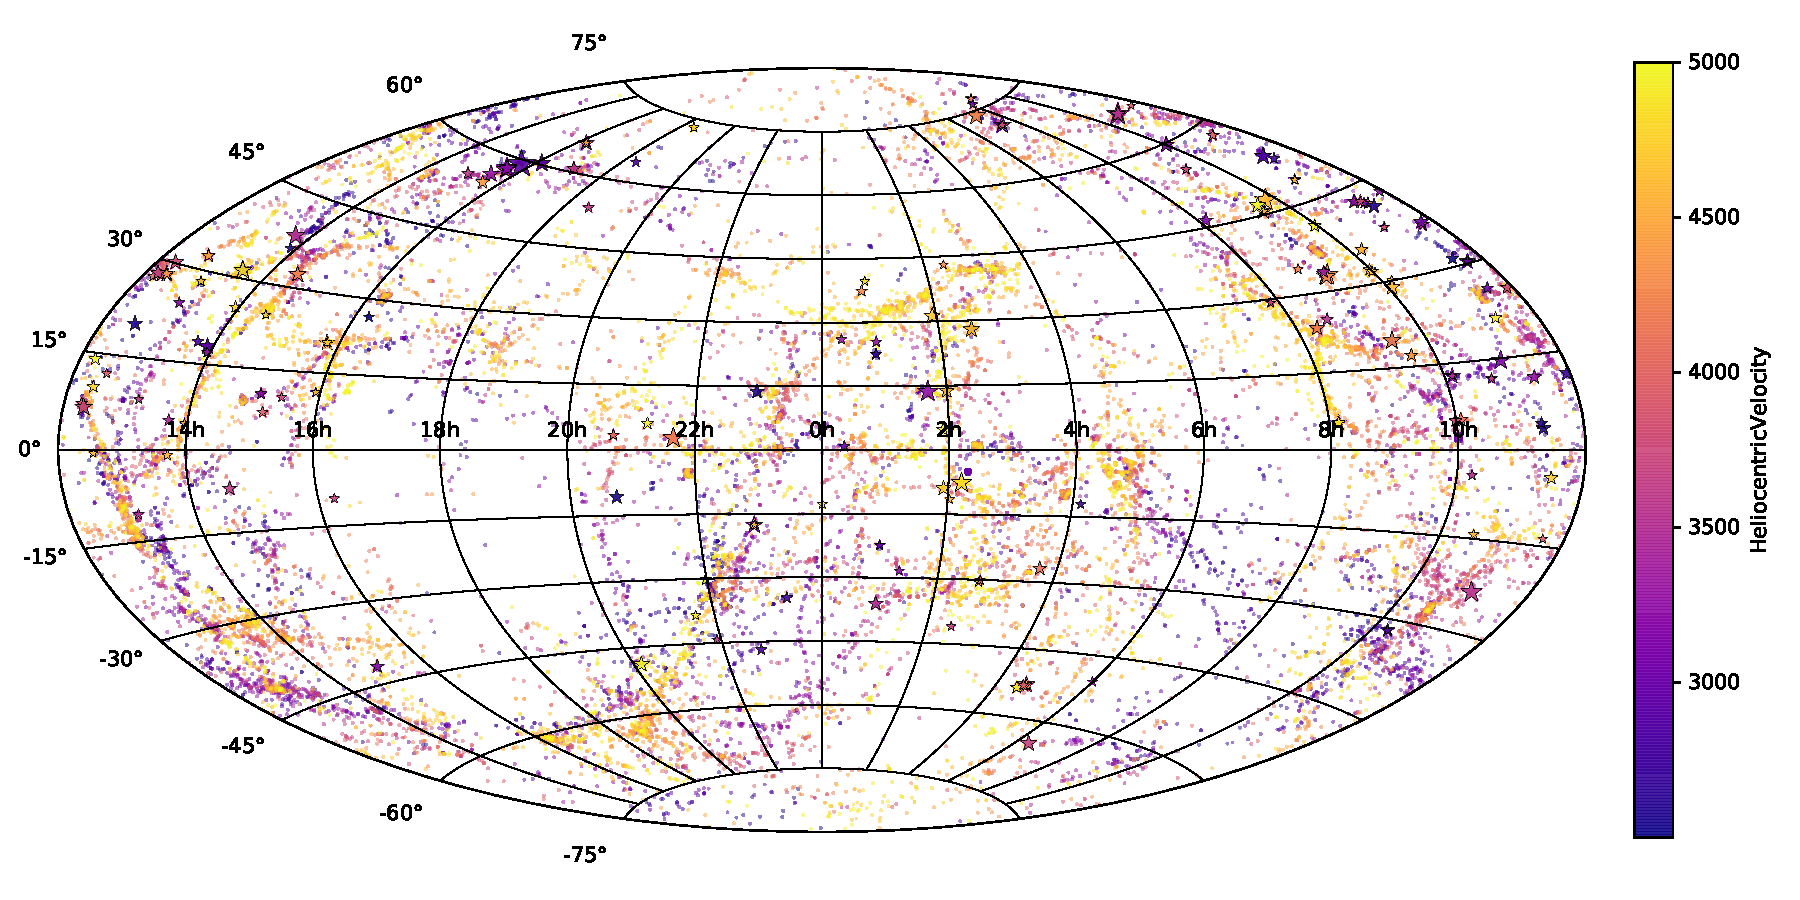
\includegraphics[width=0.99\linewidth]{5000kms_galaxies-True.pdf}}\label{allsky_5000}
  \caption{\small{All sky maps of the locations of all absorbers and galaxies. Absorbers are plotted as stars and scaled in size based on their EW. Galaxies are plotted as dots. The colors of both galaxies and absorbers are mapped to their heliocentric velocities. (a) All galaxies and absorbers in the velocity range $450 \leq cz \leq 2500$ \kms. (b) All galaxies and absorbers in the velocity range $2500 < cz \leq 5000$ \kms.}}
\vspace{0pt}
\label{allsky_2500-5000}
\end{figure*}
\begin{figure*}[ht!]
\centering
  \subfigure[]{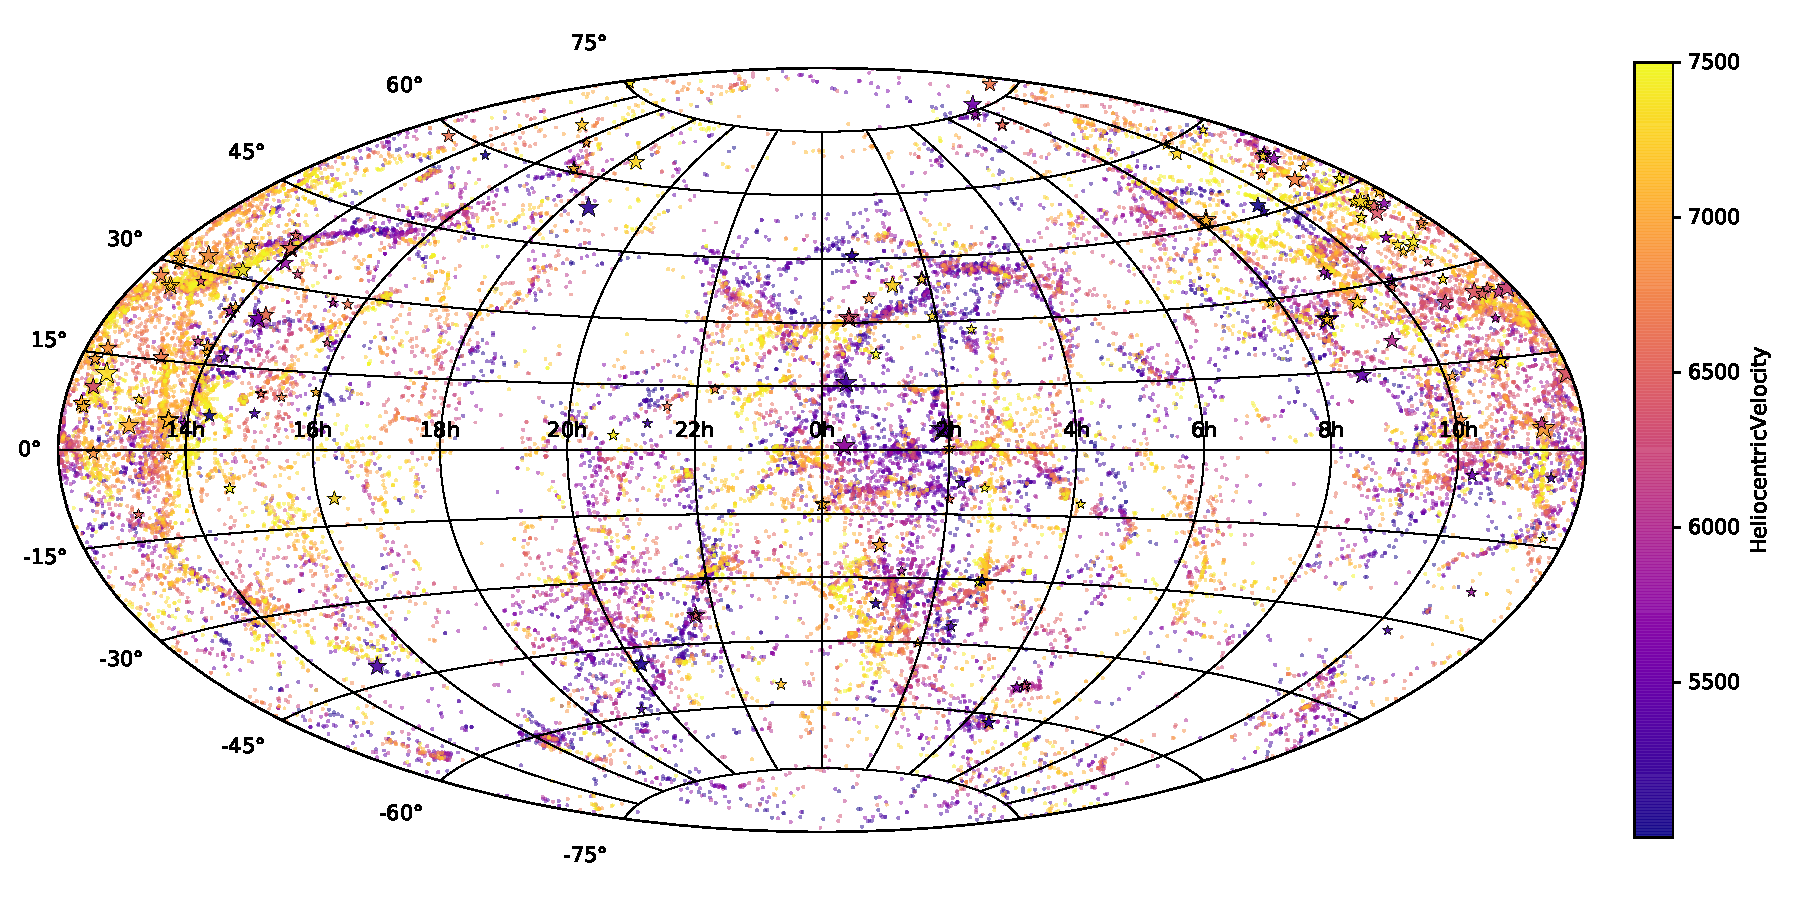
\includegraphics[width=0.99\linewidth]{7500kms_galaxies-True.pdf}}\label{allsky_7500}
  \subfigure[]{\includegraphics[width=0.99\linewidth]{10000kms_galaxies-True.pdf}}\label{allsky_10000}
  \caption{\small{All sky maps of the locations of all absorbers and galaxies. Absorbers are plotted as stars and scaled in size based on their EW. Galaxies are plotted as dots. The colors of both galaxies and absorbers are mapped to their heliocentric velocities. (a) All galaxies and absorbers in the velocity range $5000 < cz \leq 7500$ \kms. (b) All galaxies and absorbers in the velocity range $7500 < cz \leq 10,000$ \kms.}}
\vspace{0pt}
\label{allsky_7500-10000}
\end{figure*}


% this table is from pickle version 8 results
\begin{deluxetable*}{| l | c | c | c | c |}[ht!]
\setlength{\tabcolsep}{0.1in}
\tablecolumns{8}
\tabletypesize{\scriptsize}
%\tablewidth{1pt}
\tablecaption{Summary of $\mathcal{L}$ Variants \label{likelihood_variants}}
\tablehead{
\colhead{$\mathcal{L}$ Variant}  										&  \colhead{$\mathcal{L}-isolated$}	&  \colhead{$\mathcal{L}-associated-isolated$}	&  \colhead{$\mathcal{L}-associated$}	&  \colhead{$\mathcal{L}-two+$} 	}
\startdata
Total number of $\rm Ly\alpha$ absorbers: 1135 \\
571 are $isolated$ regardless of normalization \\
\hline
\hline
$\mathcal{L}_{min} = 0.01, rigor = 5$	 ($Standard$)							&	267						&	56								&	146						&	58						\\
\hline
$\mathcal{L}_{min} = 0.01, rigor = 5$, $A=2~if~\rho \leq R_{vir}$				&	267						&	56								&	160						&	55						\\
\hline
$\mathcal{L}_{min} = 0.001, rigor = 5$									&	227						&	69								&	167						&	65						\\
\hline
$\mathcal{L}_{min} = 0.001, rigor = 6$									&	227						&	69								&	162						&	68						\\
\hline
$\mathcal{L}_{min} = 0.001, rigor = 7$									&	227						&	69								&	154						&	75						\\
\hline
$\mathcal{L}_{min} = 0.001, rigor = 8$									&	227						&	69								&	145						&	78						\\
\hline
$D^{1.5}$, $\mathcal{L}_{min} = 0.001, rigor = 5$ 							&	317						&	39								&	174						&	32						\\
\hline
$\mathcal{L}_{min} = 0.001, rigor = 5$, $A=2~if~\rho \leq R_{vir}$				&	227						&	69								&	181						&	62						\\
\hline
$\mathcal{L}_{min} = 0.005$, $v_{norm} = 150, rigor = 5$						&	265						&	58								&	148						&	63						\\
\hline
$\mathcal{L}_{min} = 0.005$, $v_{norm} = 250, rigor = 5$						&	246						&	64								&	151						&	64						\\
\hline
\enddata
\tablecomments{A summary of the subset sizes resulting from varying the likelihood metric's normalization parameters. Different choices of normalization are simply shifting some of the non-$isolated$ absorbers between different bins.}
\vspace{-5pt}
\end{deluxetable*}




In this sample of 264 QSOs we have detected 1135 Ly$\alpha$ absorbers. Figures \ref{allsky_2500-5000} and \ref{allsky_7500-10000} show all-sky maps of the positions of all absorbers split into 4 velocity bins ($v_{\rm Ly\alpha} = [0 - 2500]$, $(2500 - 5000]$, $(5000 - 7500]$, and $(7500 - 10,000]$ \kms). The distribution of galaxies in the same velocity ranges are include here also (galaxies are plotted as small circles, absorbers as stars; see \textbf{Chapter 1}). Comparing the galaxy to absorber positions and velocities within each velocity range by eye, we can clearly see that the Ly$\alpha$ absorbers broadly trace the locations of the galaxies. If the current Lambda Cold Dark Matter ($\Lambda$CDM) cosmology is to be believed, this should not be remarkably surprising. The baryons from which galaxies are built and those found within the IGM and traced by $\rm Ly\alpha$ absorption should both follow the underlying potential produced by the Dark Matter, and should therefore be found in similar places. Beyond this big-picture result however, we want to know how the absorbers react to the presence of the galaxies on a more local scale.


\subsection{Sub-sample selection}
A major hurdle for galaxy-absorber correlation studies has always been matching any particular absorption line to a single nearby galaxy. The basic premise of matching relies on the assumption that, in at least some cases, one particular galaxy's potential, angular momentum, and radiation field dominates what an absorber ``feels" (i.e., is the primary influencer for the EW, column density and Doppler $b$-parameter of an absorber). With this assumption in place, the issue becomes that galaxies are generally not isolated. When faced with a distribution of galaxies of differing types, sizes, orientations and distances (impact parameters) and velocities ($\Delta v = v_{\rm absorber} - v_{\rm galaxy}$) from an absorption line, which, if any, are most likely to be ``associated" with the line? 

As first introduced in \cite{french2017}, we employ a unique likelihood method for objectively matching absorbers with nearby galaxies in a consistent, analytical manner. We define likelihood, $\mathcal{L}$, as follows: 

\begin{equation}
\mathcal{L} = A \times e^{-(\frac{\rho}{R_{\rm eff}})^2} \times e^{-(\frac{\Delta v}{v_{\rm norm}})^2},
\label{likelihood}
\end{equation}

\noindent where $A$ is a normalization constant, $\rho$ is the impact parameter between a galaxy and sightline, $R_{\rm eff}$ is one of two possible ``effective - radii" we use for galaxies (virial radius and $D^{1.5}$, or diameter to the 1.5 power), $\Delta v$ is the velocity separation between absorber and galaxy heliocentric, and $v_{\rm norm}$ is a velocity normalization (equal to one of 150, 200, or 250). 

We calculate $\mathcal{L}$ for every absorber-galaxy combination, which then gives us a single number as a three-dimensional proxy for the physical separation between the two. Based on this $\mathcal{L}$ we then separate our sample into the following 5 distinct bins: $isolated$, $\mathcal{L}-isolated$, $\mathcal{L}-associated-isolated$, $\mathcal{L}-associated$, and $\mathcal{L}-two+$. The $isolated$ sample contains all the $\rm Ly\alpha$ lines that are farther than 500 kpc and 400 \kms~from \emph{any} galaxy. The $\mathcal{L}-isolated$ sample contains those $\rm Ly\alpha$ lines are far enough away from any galaxy so as to not meet our minimum-$\mathcal{L}$ criteria. The $\mathcal{L}-associated-isolated$ sample contains those $\rm Ly\alpha$ lines which meet our $\mathcal{L}$ criteria to be associated with a single galaxy, and that galaxy is isolated by 500 kpc and 400 \kms. The $\mathcal{L}-associated$ sample contains those $\rm Ly\alpha$ lines which meet our $\mathcal{L}$ criteria to be associated with a single galaxy, but that galaxy is \emph{not} isolated. And finally, the $\mathcal{L}-two+$ sample contains those  $\rm Ly\alpha$ lines which meet our minimum-$\mathcal{L}$ criteria to be associated with \emph{more} than one galaxy.

Our standard criteria for a positive galaxy-absorber association are $\mathcal{L} \geq 0.01$ and $\mathcal{L}_1 \geq rigor \times \mathcal{L}_2$ with $rigor =5$ (i.e., the $\mathcal{L}$-value for the most likely associated galaxy must be at least 5 times greater than that for the second most likely galaxy). However, we have also explored the results of adjusting the several possible $\mathcal{L}$ normalizations. We calculate $\mathcal{L}$ with $R_{\rm eff}$ equal to $R_{\rm vir}$ and $D^{1.5}$ and $v_{\rm norm}$ equal to 150, 200, and 250. For each of these combinations, we also calculate a variant with $A =1$ and another with $A = 2$ if $R_{\rm eff} \ge \rho$, and $A=1$ otherwise. Additionally, we investigate the effect of changing the minimum-$\mathcal{L}$ criteria to 0.005 and 0.001, and $rigor$ = 5, 6, 7, and 8. Table \ref{likelihood_variants} summarizes the resulting subsets for each of these combinations. Overall, we find that none of these adjustments have a major effect on the resulting samples. For the remainder of this analysis we will concentrate on the $\mathcal{L}_{\rm min} = 0.01, v_{\rm norm} = 20$, $A = 2$ normalization subsets. This matches the normalization we adopted in \cite{french2017}, and represents a middle ground option while also maximizing the size of the $\mathcal{L}-isolated-associated$, $\mathcal{L}-associated$, and $\mathcal{L}-two+$ subsets. \textbf{MORE}

%For the remainder of this analysis we will concentrate on the $\mathcal{L}_{\rm min} = 0.005, v_{\rm norm} = 250$ normalization subsets. This represents a middle ground option while also maximizing the size of the $\mathcal{L}-isolated-associated$, $\mathcal{L}-associated$, and $\mathcal{L}-two+$ subsets. \textbf{MORE}


%($A=1$, $R_{eff} = R_{vir}$, $v_{norm} = 200$, $\mathcal{L}_{min} = 0.01$)


\section{Results \& Discussion}

First we explore the $\rm Ly\alpha$ detection fraction as a function of galaxy proximity. To calculate this, we start by correlating the position of every QSO with our galaxy sample. For every galaxy found within 1000 kpc in physical impact parameter of each sightline we then check if a $\rm Ly\alpha$ line appears in that sightline and within 400 \kms~of the galaxy's systemic velocity. This results in a detection fraction as a function of impact parameter. Additionally, we calculate the detection fraction as a function of likelihood, $\mathcal{L}$, in a similar manner. However, as we are calculating detection fraction without any a priori knowledge of the velocity of the absorption lines, the likelihood function we use is modified from Eq. \ref{likelihood} to simply $e^{-(\rho/R_{vir})^2}$, or only the impact parameter - virial radius portion of our usual likelihood function given by Eq. \ref{likelihood}. Note that this adjusted likelihood function is identical to Eq. \ref{likelihood} when $\Delta v = 0$. 

\begin{figure}[t!]
        \centering
        \vspace{0pt}
        \includegraphics[width=0.49\textwidth]{detection_fraction_both_err.pdf}
        \caption{\small{The detection fraction as a function of impact parameter (grey-circles) and $\mathcal{L}$ (blue-diamonds). Note that the impact parameter and $\mathcal{L}$ $x$-axis scales are quite different; the lowest $\mathcal{L}$ bin (0.0001) corresponds to $\sim 3 R_{\rm vir}$, whereas the largest impact parameter bin (1000 kpc) is generally $\gg 3 R_{\rm vir}$. Error bars show the $1\sigma$ Poisson errors.}}
        \vspace{5pt}
        \label{detection_fraction}
\end{figure}

We have plotted the detection fraction as a function of both impact parameter and $\mathcal{L}$ in Figure \ref{detection_fraction}. As expected, the detection fraction clearly increases with decreasing impact parameter and increasing $\mathcal{L}$. However, while the detection fraction continues to rise all the way to the 25 kpc mark however, it levels off at $\sim 1.5 R_{\rm vir}$ ($\sim 0.1 \mathcal{L}$) as a function of likelihood. \textbf{WHY? MORE}


\subsection{Equivalent Width}

Here we explore the effect of environment on the equivalent width of our $\rm Ly\alpha$ absorber sample. Figure \ref{cdf_ew} shows the cumulative distribution function of equivalent widths for each of our 5 likelihood-separated subsets, along with that of the entire sample in black). We have only included $\rm EW \ge 50~m\AA$ here to mitigate any bias due to the detection limit of lower-SN targets. We find that each subset occupies a distinct space aside from the $\mathcal{L}-associated-isolated$ and $\mathcal{L}-associated$ sets, which are essentially indistinguishable. The physical result of this is that the strength EW of $\rm Ly\alpha$ absorption depends strongly on environment. Stronger absorption lines are preferentially found near to galaxies, and the strongest lines are found near multiple galaxy systems. The result of Anderson-Darling statistical distribution tests between each subset indicate that our $isolated$ and $\mathcal{L}-isolated$ subsets are distinct from each of $\mathcal{L}-two+$, and $\mathcal{L}-associated-isolated$ and $\mathcal{L}-associated$ at a $>95\%$ confidence level. Because $\mathcal{L}-associated-isolated$ and $\mathcal{L}-associated$ are found to be nearly indistinguishable via these test and by-eye, we will combine them for the remainder of this analysis.

\begin{figure}[t!]
        \centering
        \vspace{15pt}
        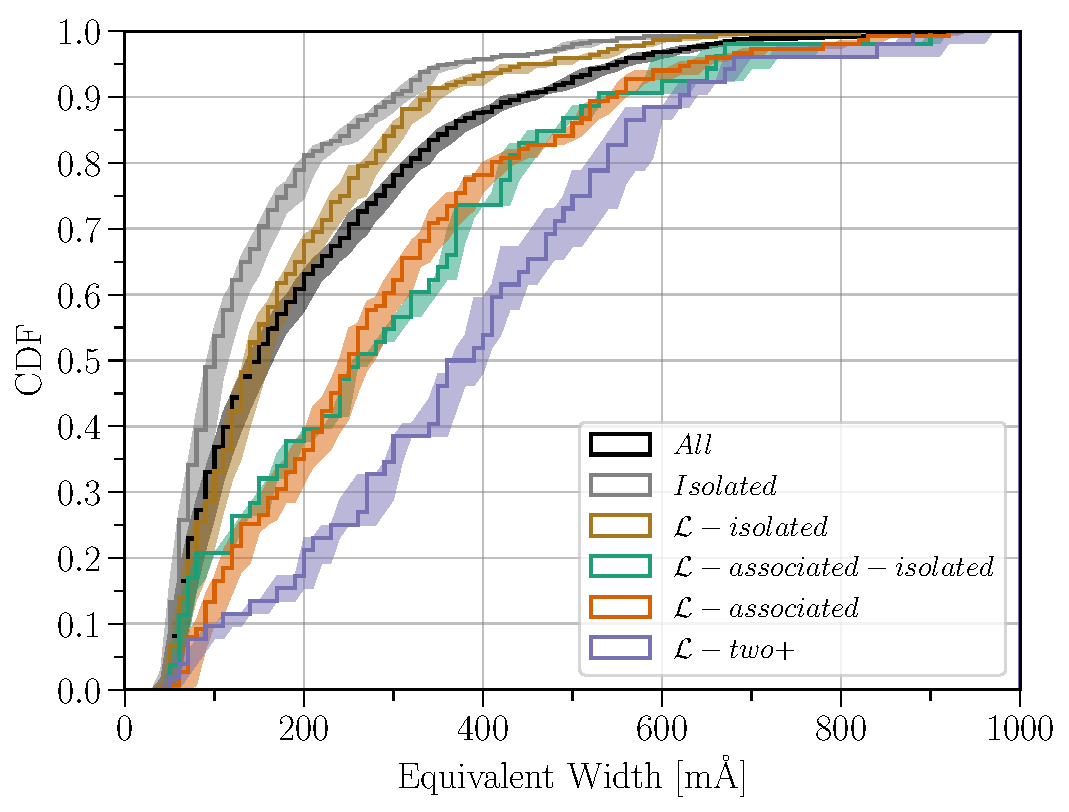
\includegraphics[width=0.49\textwidth]{hist(EW)_bins10_6_EWcut50-15000_err_dataset_double.pdf}
        \caption{\small{The equivalent width (EW) cumulative distribution function for each subset of our Ly$\alpha$ absorber sample. From the top-left corner to the bottom-right the curves are the fully isolated absorbers (grey), the absorbers isolated enough from any galaxy to not be likelihood-matched (brown), the full distribution (black), the absorbers likelihood-matched to a single, non-isolated galaxy (orange), the absorbers matched to a single, isolated galaxy (green), and the absorbers likelihood-matched with two or more galaxies (purple). The shaded region around each curve gives the EW measurement errors. Only $\rm EW \ge 50~m\AA$ absorbers are included to mitigate any bias due to the detection limit of lower-SN targets.}}
        \vspace{5pt}
        \label{cdf_ew}
\end{figure}

This separation between EW distributions based on galaxy proximity is likely an effect of the distribution of the cosmic web; multiple galaxies should form from denser sections and intersections of intergalactic filaments, and these environments should thus also produce a stronger absorption profile. 


\begin{figure*}[t!]
        \centering
        \vspace{0pt}
        \subfigure[]{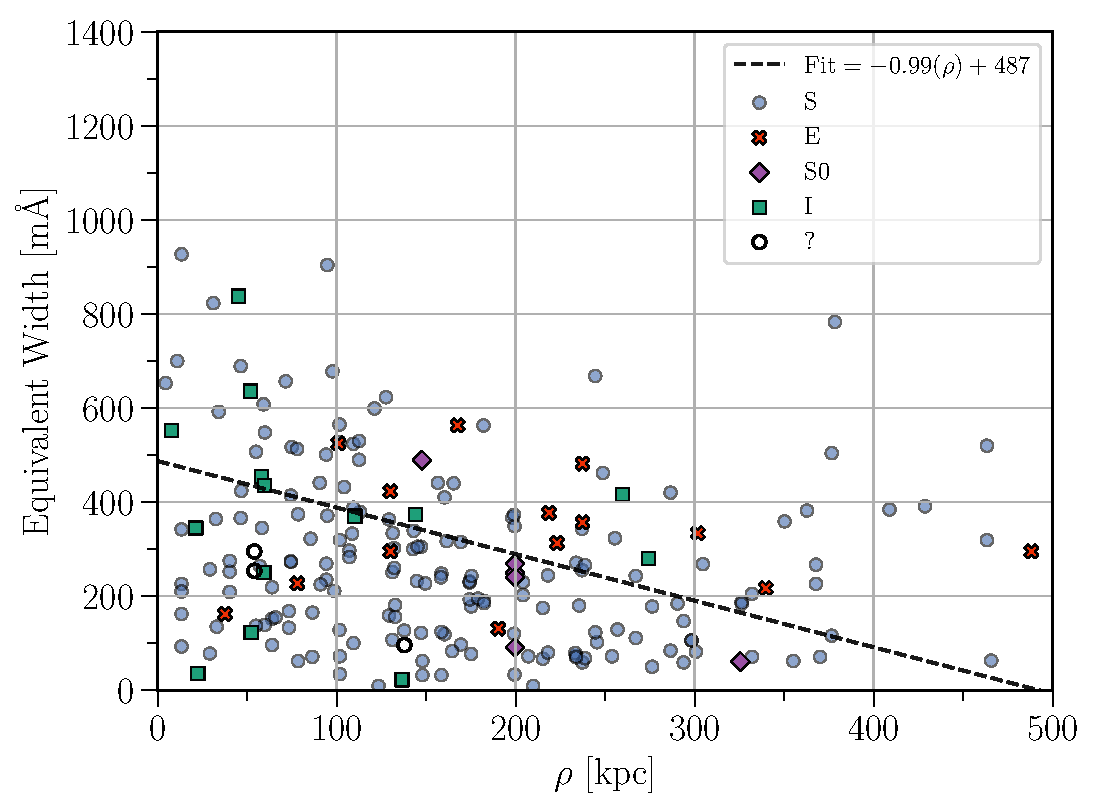
\includegraphics[width=0.49\textwidth]{W(impact)_MType_binSize50_EWcut0-10000_dataset_double.pdf}\label{ew_impact}}
        \subfigure[]{\includegraphics[width=0.49\textwidth]{W(impact_vir)_MType_binSize0_5_EWcut0-10000_dataset_double.pdf}\label{ew_impact_rvir}}
        \caption{\small{\textbf{Left: } The equivalent width (EW) of absorbers a function of impact parameter ($\rho$) to the associated galaxy. The best fit shown by the dashed-black line has the form: $EW = m (\rho) + b,$ with $m = -0.99 \pm 0.25$ and $b = 487 \pm 49$. \textbf{Right:} The EW of absorbers a function of impact parameter to the associated galaxy normalized by the galaxy virial radius ($\rho / R_{\rm vir}$). The best fit shown by the dashed-black line has the form: $EW = m (\rho / R_{\rm vir}) + b,$ with $m = -265 \pm 48$ and $b = 620 \pm 59$. \textbf{Both:} All $\mathcal{L}-associated-isolated$ and $\mathcal{L}-associated$ systems are included here. Blue-circles indicate spiral-type galaxies, green-squares indicate irregulars, red-crosses indicate ellipticals, purple-diamonds indicate S0's, and open black-circles indicate ambiguous morphological types. }}
        \vspace{5pt}
        \label{ew_both}
\end{figure*}

This result on it's own does not however illuminate any deeper connection or relationship between the individual galaxies and absorbers. Let us now consider the dependence of EW on galaxy impact parameter, as illustrated in Figure \ref{ew_impact}. We have also plotted EW as a function of virial radius normalized impact parameter ($\rho/ R_{\rm vir}$) in Figure \ref{ew_impact_rvir}. Firstly, we notice that weak ($\rm EW \lesssim 400~m\AA$) absorbers are found at all impact parameters and $\rho / R_{\rm vir}$, which agrees with our findings above from Figure \ref{cdf_ew}. Moreover, absorbers stronger than $\rm EW \sim 400~m\AA$ are preferentially found close to galaxies, and absorbers with $\rm EW \sim 800~m\AA$ are \emph{only} found within 100 kpc and $1 R_{\rm vir}$. Hence, weak $\rm EW \lesssim 400~m\AA$ absorbers are most likely $\rm Ly\alpha$-forest material, while the stronger absorbers are associated with the galaxies.

Secondly, we have included linear fits in both Figures \ref{ew_impact} and \ref{ew_impact_rvir} as shown by the dashed-black lines. In each case we find a strong negative slope, and by eye the virial radius normalized version appearing to be the stronger correlation. To test this we calculated the Pearson correlation coefficient $r$-value for each fit. For the purely impact parameter correlation we find a Pearson $r$-value $=-0.26$, with a $p$-value of $p = 1.2 \times 10^{-4}$, which indicates a weak but statistically significant negative correlation. For the virial radius normalized correlation we find $r = -0.35$ with $p = 1.2 \times 10^{-7}$, indicating a stronger and \emph{more significant} negative correlation. If true, then the EW of $\rm Ly\alpha$ absorption depends on the size of galaxy halos. Hence, either the physical or number density (or both) of absorbing cloudlets is greater closer to galaxies in a halo-scale dependent manner. The increased density of this neutral material could signify both inflows or outflows from galaxies, with inflows expected to harbor a greater fraction of the cool, neutral \HI~most readily traced by $\rm Ly\alpha$. An analysis of metals associated with these neutral cloudlets could provide clues to which is the mechanism source at play here.

Thirdly, let us consider the affect of galaxy morphology on the associated absorption, which we have indicated in Figure \ref{ew_both} by the color and style of the plot points. In each figure blue-circles indicate spiral-type galaxies, green-squares indicate irregulars, red-crosses indicate ellipticals, purple-diamonds indicate S0's, and open black-circles indicate ambiguous or unknown types. Spiral galaxies are clearly the dominant type, and are found at all impact parameter and EW. \textbf{WHAT FRACTION OF ALL GALAXIES ARE SPIRAL VS E?}. Irregulars are the next most common, but are not spread around as evenly. All but two irregular-type systems are separated by less than 150 kpc in Figure \ref{ew_impact}, and few low-EW absorbers are found within $\sim 0.5 R_{\rm vir}$ in Figure \ref{ew_impact_rvir}. In the first case, this can be explained by irregulars having a smaller average size ($\overline{R}_{\rm vir} = 101$ kpc for irregulars, compared to 145, 178, and 194 kpc for spirals, S0's, and ellipticals). When normalized by virial radius however, the lack of low-EW absorbers at low $\rho / R_{\rm vir}$ could be an indication of more gas-rich halos. This would make sense, since irregular galaxies are often tidally disturbed due to recent interactions which can result in extended, gas-rich halos.

Finally, we also see that elliptical and S0 galaxies are associated with mostly low-EW absorption, especially within 100 kpc and $\sim 0.5 R_{\rm vir}$. \textbf{MORE}



\subsection{Doppler b-parameter}

Here we explore the effect of environment on the Doppler $b$-parameter of our $\rm Ly\alpha$ absorber sample. In an analogous fashion as above, Figure \ref{cdf_b} shows the cumulative distribution functions for the Doppler $b$-parameters of each subset of absorbers. Like the EW result, the Doppler $b$-parameters trend toward larger values based on their proximity to galaxies. The separation here is weaker, but the separation between, e.g., Isolated and $\mathcal{L}-Two+$ samples, remains statistically significant.

\begin{figure}[ht!]
        \centering
        \vspace{0pt}
        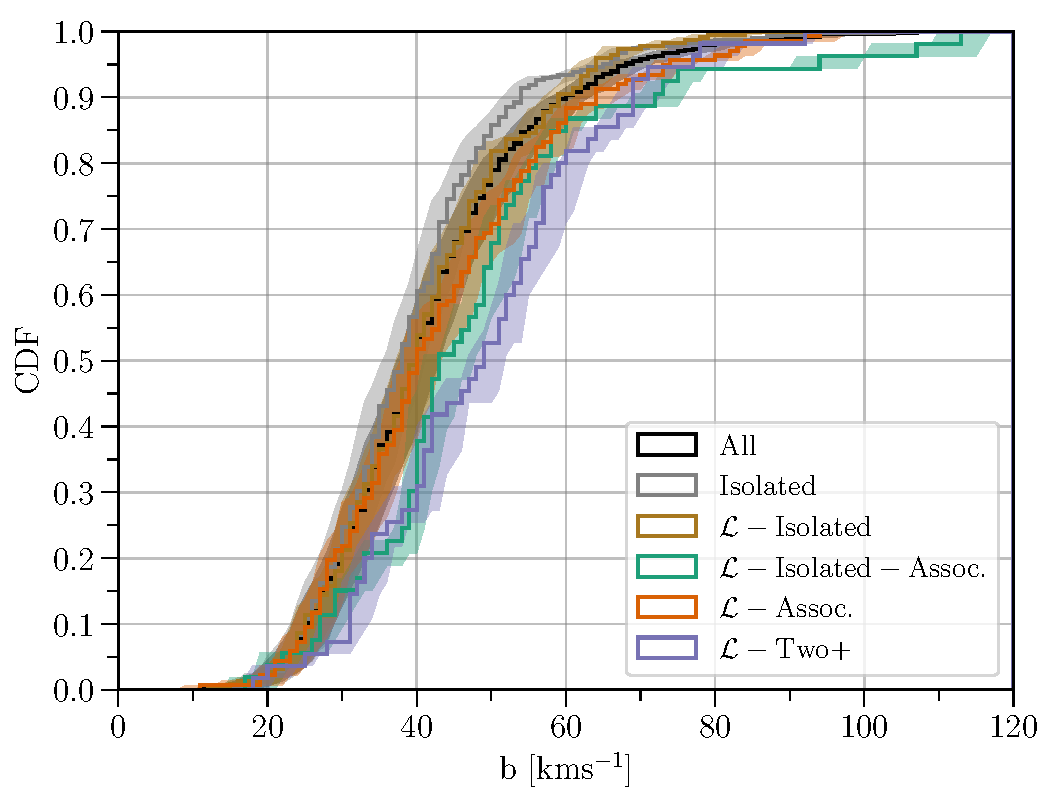
\includegraphics[width=0.49\textwidth]{hist(b)_all6_bins1_EWcut50-10000_errTrue_dataset.pdf}
        \caption{\small{The Doppler $b$-parameter ($b$) cumulative distribution function for each subset of our Ly$\alpha$ absorber sample. From the top-left corner to the bottom-right the curves are the fully isolated absorbers (grey), the absorbers isolated enough from any galaxy to not be likelihood-matched (brown), the full distribution (black), the absorbers likelihood-matched to a single, non-isolated galaxy (orange), the absorbers matched to a single, isolated galaxy (green), and the absorbers likelihood-matched with two or more galaxies (purple). The shaded region around each curve gives the $b$-parameter measurement errors. Only $\rm EW \ge 50~m\AA$ absorbers are included to mitigate any bias due to the detection limit of lower-SN targets.}}
        \vspace{5pt}
        \label{cdf_b}
\end{figure}



\subsection{Azimuth}
Here we investigate the dependence of $\rm Ly\alpha$ absorber properties on their orientation with respect to the major axis of nearby galaxies. It is commonly expected that gas found near the major axis of a galaxy represents accreting material, while material around the minor axis represents outflows \textbf{CITE??}. 



\subsection{Inclination}

Here we investigate the inclination dependence of $\rm Ly\alpha$ absorber properties.

As expected if this is the case, we also see an inclination dependence in the overall $\rm Ly\alpha$ detection fraction. For example, if absorbers are distributed in a perfectly spherical manner around galaxies, then we would expect just as many non-detections as detections at any given galaxy inclination and impact parameter from a sightline. We do not find this. Figure \ref{detection_fraction_inclination} shows the median inclinations for galaxies near positive or negative $\rm Ly\alpha$ detections as a function of both impact parameter and $\mathcal{L}$. In both cases, positive detections are predominantly found near more highly inclined galaxies than non-detections.



\begin{figure*}
\centering
  \subfigure[]{\includegraphics[width=0.49\linewidth]{detection_fraction_impact_inc_median_Lstarcut01-2.pdf}\label{detection_fraction_impact_inc}}
  \subfigure[]{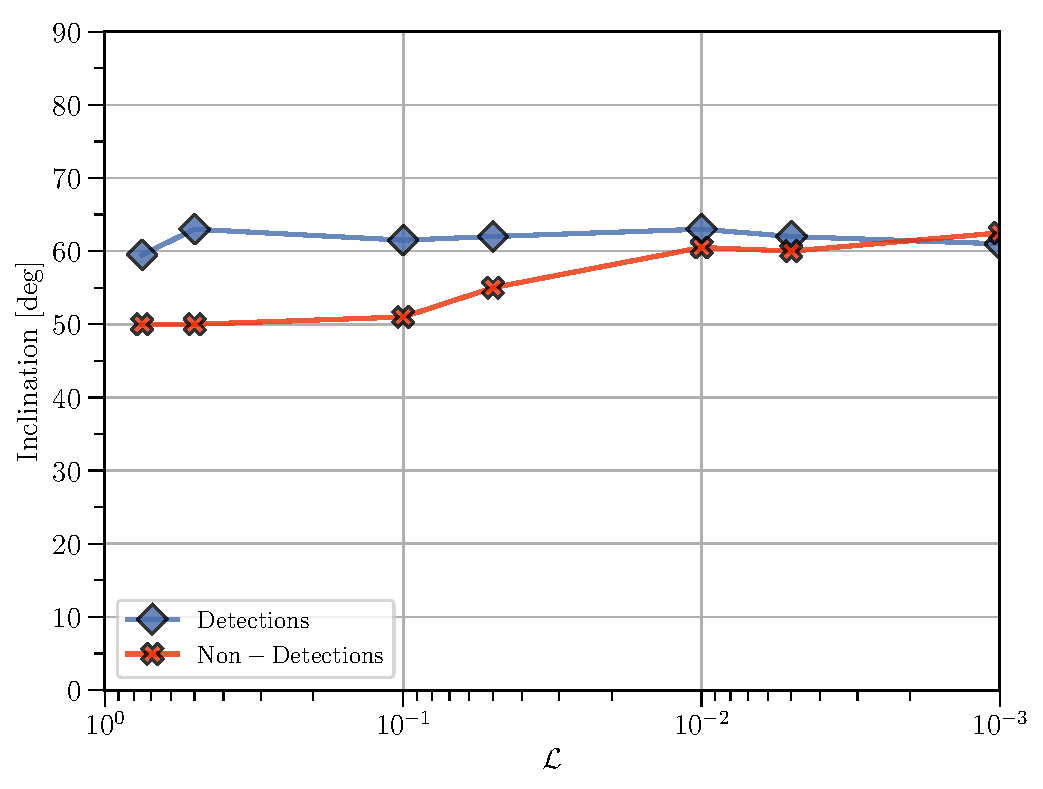
\includegraphics[width=0.49\linewidth]{detection_fraction_likelihood_inc_median_Lstarcut01-2.pdf}\label{detection_fraction_likelihood_inc}}
  \caption{\small{(a) The median inclination is shown for galaxies at a given impact parameter from a positive (blue-diamonds) or negative (red-crosses) $\rm Ly\alpha$ detection. (b) The median inclination is shown for galaxies at a given $\mathcal{L}$ from a positive (blue-diamonds) or negative (red-crosses) $\rm Ly\alpha$ detection.}}
  \label{detection_fraction_inclination}
\vspace{0pt}
\end{figure*}


\section{SUMMARY}
1. $\rm Ly\alpha$ absorbers with $\rm EW \lesssim 100 m\AA$ are ubiquitous, making up nearly $50\%$ of all $\rm Ly\alpha$ systems in the nearby Universe, and do not correlate strongly with environment ($70\%$ of these weak absorbers are isolated). 




\section{Future Work}

We have established large, rich dataset with which to explore the relationship between circumgalactic material and the galaxies that reside in it. Much can still be learned by continuing to delving deeper into this data. The first future goal we have is to produce galaxy-$\rm Ly\alpha$ two-point cross-correlation functions, as has been demonstrated by, e.g., \cite{chen2005}, among others. This will be our first goal as it does not involve any significant additions to the data already presented here.

Our next goal will be to produce Voigt profile fits for each absorber. While equivalent widths and second-moment derived $b$-parameters are an incredibly convenient and powerful tool to study



Perhaps the most obvious 


Cross-correlation functions \cite{chen2005}

Metals





%%\begin{eqnarray}
%%	\nonumber
%%	\sigma^2 = \left( \frac{\partial v_{rot}}{\partial \lambda_{obs}} \right)^2 (\Delta \lambda_{obs})^2 + \\
%%	\nonumber
%%	\left(\frac{\partial v_{rot}}{\partial v_{sys}} \right)^2 (\Delta v_{sys})^2 + \\
%%	\left( \frac{\partial v_{rot}}{\partial i} \right)^2 (\Delta i)^2,
%%\end{eqnarray}



\acknowledgements

This research has made use of the NASA/IPAC Extragalactic Database (NED) which is operated by the Jet Propulsion Laboratory, California Institute of Technology, under contract with the National Aeronautics and Space Administration. Based on observations with the NASA/ESA \textit{Hubble Space Telescope}, obtained at the Space Telescope Science Institute (STScI), which is operated by the Association of Universities for Research in Astronomy, Inc., under NASA contract NAS 5-26555. Spectra were retrieved from the Barbara A. Mikulski Archive for Space Telescopes (MAST) at STScI. Over the course of this study, D.M.F. and B.P.W. were supported by grant XXXX

%AST-1108913, awarded by the US National Science Foundation, and by NASA grants \textit{HST}-AR-12842.01-A, \textit{HST}-AR-13893.01-A, and \textit{HST}-GO-14240 (STScI). 

\facility{HST (COS)}
\clearpage

%\nocite{*}
%\bibliography{rotation_bib}
%\bibliography{/Users/frenchd/Research/bib}{}
\bibliography{/Users/frenchd/Research/inclination/git_inclination/bib}{}
\bibliographystyle{apj}

\clearpage

\appendix

\end{document}
